% -*- TeX:SI -*-
% slovene sub-mode for spell check



\chapter{Varnost pri delu z industrijskimi roboti}

Industrijski robot je pozicijsko vodena, programabilna in
večopravilna naprava, ki se giblje vzdolž več prostostnih stopenj v
prostoru. Namenjen je manipulaciji materiala, obdelovancev in orodij
pri izvajanju različnih delovnih nalog in programiranih gibov.

Glede na zagotavljanje varnosti uvajanje industrijskih robotov v
proizvodnjo predstavlja dva nasprotna si vidika. Na eni strani
uporaba industrijskih robotov v nevarnem in človeku škodljivem
okolju povečuje človekovo varnost. Uporaba robotov za avtomatsko
varjenje, kovanje, peskanje, barvanje, itd. omogoča, da je človek
umaknjen iz neprijaznega in nevarnega delovnega okolja. Na drugi
strani pa lahko roboti med obratovanjem sami ogrožajo varnost
delavcev. Pri delu z roboti so možni nesrečni slučaji, lahko tudi
tragični, če ni ustrezno poskrbljeno za zagotavljanje varnosti.

Glavna nevarnost pri delu z roboti na človeka preti v robotovem
delovnem prostoru. Robot je sposoben prostega gibanja v širokem
prostoru, sposoben je hitrih nepredvidenih gibov in nagle
spremembe konfiguracije. Navedeno lahko predstavlja neposredno
ogrožanje varnosti osebe, ki dela ali stoji v bližini robota. Zato
je potrebno pri vsaki robotski celici oceniti kakšno je tveganje
za varnost in uvesti ukrepe za zmanjšanje možnosti nesreč.

Nepričakovano gibanje robota lahko povzroči okvara sistema ali
človeška napaka. Med te prištevamo:
\begin{itemize}
    \item \vspace*{-0.1cm} Nepredvideno obnašanje robota, katerega vzrok je
    napaka v robotskem krmilnem sistemu.
    \item \vspace*{-0.1cm} Prekinitev pomembnih kabelskih povezav, ki je posledica
    robotskega gibanja.
    \item \vspace*{-0.1cm} Napaka pri prenosu podatkov, ki povzroči večji gib robota
    od pričakovanega.
    \item \vspace*{-0.1cm} Napaka ali okvara delovanja orodja npr.
    varilne pištole.
    \item \vspace*{-0.1cm} Programske napake ali druge napake v delovanju.
    \item \vspace*{-0.1cm} Premajhna preciznost gibanja ali izraba.
    \item \vspace*{-0.1cm} Nekompatibilnost vpenjal in drugih orodij.
\end{itemize}

\section{Nevarnosti pri delu z roboti}

V osnovi obstajajo tri potencialne nevarnosti pri delu z
industrijskimi roboti:
\begin{itemize}
    \item \vspace*{-0.1cm} Nevarnost trka, ki je možnost, da gibajoči se robot ali
    orodje, ki ga robot nosi, zadane operaterja. Trk je lahko posledica
    nepričakovanega giba robota ali izmeta/izpustitve
    obdelovanca.
    \item \vspace*{-0.1cm} Nevarnost stisnjenja je nevarnost, da robot med gibanjem v bližini objektov,
    ki so fiksni, kot npr. stroji, oprema, ali ograja, stisne
    operaterja. Nevarnost stisnjenja obstaja tudi pri delu ob
    vozičkih, tekočih trakovih, paletah in drugih
    transportnih mehanizmih.
    \item \vspace*{-0.1cm} Ostale nevarnosti, ki so specifične posamezni robotski aplikaciji, kot npr.
    nevarnosti
    udara električenga toka, vplivov varilnega obloka,
    opeklin, strupenih snovi, sevanja, prekomernega zvoka, itd.
\end{itemize}

\begin{figure}[h]
\centering
\resizebox{10cm}{!}{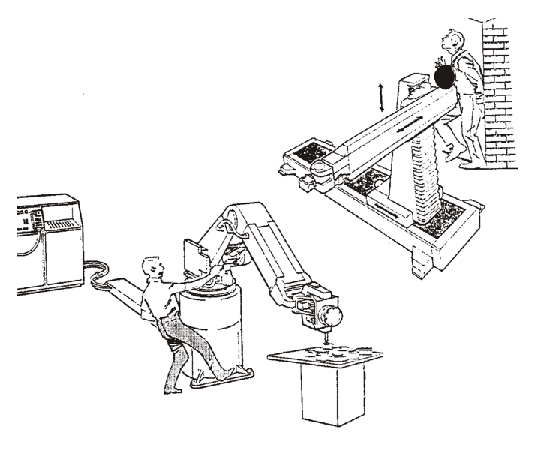
\includegraphics[draft=false]{nevarnosti.eps}}
\caption{\label{cop}Nevarnost trka in nevarnost stisnjenja pri
delu z industrijskimi roboti}
\end{figure}

Gornje nevarnosti izvirajo iz naslednjih vzrokov:
\begin{itemize}
    \item \vspace*{-0.1cm} \textbf{Nevarnosti krmilnega sistema:} To
    so nevarnosti napak, ki se dogode v robotskem krmilniku, kot
    so npr. programske napake, napake zaradi interference signalov ter napake v
    hidravličnih, pnevmatskih ali električnih podsistemih povezanih z robotom.
    \item \vspace*{-0.1cm} \textbf{Mehanske nevarnosti:} V ta
    razred sodijo nevarnosti, ki so posledica mehanskih lastnosti
    obdelovancev ali orodij, ki jih prenaša robot. Te so npr. ostri
    robovi, večje mase ali nezastrte elektrode. Zaradi mehanskih
    napak lahko robotsko prijemalo nepredvideno izpusti
    obdelovanec. Vzroki mehanskih napak so prekomerna obremenitev,
    korozija, utrujanje materiala in pomanjkljivo vzdrževanje.
    \item \vspace*{-0.1cm} \textbf{Nevarnosti okolja:} Uporaba
    robotov lahko v določenih situacijah povzroči tudi tveganja iz
    okolja. Tovrsten primer so varilne robotske celice od katerih
    se širijo varilni plini, varilno iskrenje ter leteči delci.
    Podobno tveganje predstavljajo tudi prah, vlaga, ionizirajoče in neionizirajoče
    sevanje, laserski žarki, ultraviolična svetloba ter gorljivi in
    eksplozivni plini.
    \item \vspace*{-0.1cm} \textbf{Nevarnosti človeških napak:} V
    večini robotskih celic mora operater delati v bližini robota
    ali vstopati v njegov delovni prostor. V tem primeru je
    izpostavljen nevarnosti trka ali stisnjenja, ki lahko nastopi
    med programiranjem, učenjem gibanja, vzdrževanjem, ali delom v
    bližini robota npr. vlaganjem ali jemanjem obdelovancev iz
    celice. Slabo poznavanje opreme je glavni vzrok za človeške napake pri delu z roboti.
    \item \vspace*{-0.1cm} \textbf{Nevarnosti perifernih naprav:}
    V večini robotskih celic robot dela v povezavi s perifernimi
    enotami, kot so obdelovalni stroji, tekoči trakovi,
    obdelovalna orodja, stiskalnice, itd. Tovrstna oprema prav tako
    lahko predstavlja varnostno tveganje, če so nevarni deli v
    dosegu operaterja in niso zaščiteni z varnostnimi ograjami.
\end{itemize}

Poročila o nesrečah z industrijskimi roboti odkrivajo, da se
večino nesreč dogodi, ko operater vstopi v robotski delovni
prostor potem, ko se je robot predhodno ustavil ali se gibal
počasi, nenadoma pa se je začel gibati in hitro pospeševati.

\clearpage
\section{Zahteve in zagotavljanje varnosti pri delu z roboti}

 \vspace{5mm}

\textbf{Splošne zahteve za varno delovanje industrijske strojne
opreme} predvidevajo, da morajo biti vsi gibajoči se deli opreme,
vsak del prenosnih sistemov in vsak nevaren del varno zakriti.
Izjeme obstajajo v primerih, ko so ti deli v takšnem položaju ali so
takšne konstrukcije, da so že sami po sebi varni kot da bi bili
zakriti. Smernice za varno delovanje strojev so podane v direktivah
o strojih 98/37/EC in 2006/42/EC. Pri klasičnih strojih so nevarni
deli običajno vgrajeni v njegovi notranjosti. Delovanje strojev je
pod popolno kontrolo človeka in so zato vzroki nesreč večinoma
pripisani človeškemu faktorju. V nasprotju s stroji, pa je pri
robotski celici lahko potencialno nevarna širša okolica robota, ki
obsega celoten robotov delovni prostor, pa tudi bližnjo okolico v
primeru letečih delcev ali kosov. Zaradi tega je potrebno skrbno
preučiti do kod sega področje nevarnosti in tega ustrezno zaščititi.
Pri tem je pomembna analiza potencialnih nevarnosti, ki mora biti
izvedena na sistematični način. Standard, ki ureja varno delovanje
robotskih celic, je novejši standard ISO 10218 (ang. naslov: Robots
for industrial enviroments - Safety requirements). Standard ni
obvezujoč, saj daje le praktična priporočila za zagotavljanje
varnega delovanja. Robotska celica, ki je zgrajena gleda na
priporočila, hkrati ustreza tudi direktivi o strojih.


\subsection{Zagotavljanje varnosti na nivoju strojne opreme}

 \vspace{5mm}

 \textbf{Varnostna zaščita} se glede na priporočila standarda
 EN 954-1:1999 (ang. naslov: Safety of machinery, Safety-related parts of
 control systems, Part 1: General principles for design, ki je
 harmoniziran ISO 13849-1:1999) lahko izvaja na treh nivojih:

\begin{description}
       \item \textbf{Nivo 1} je nivo varovanja obsega celotne robotske
       celice. Običajno je varovanje izvedeno s fizičnim
       ograjevanjem s pomočjo kombinacije mehanskih ograj in vrat.
       Kot opcija so lahko uporabljene tudi naprave za zaznavanje prisotnosti
       ter zvočne in svetlobne opozorilne naprave, vendar le kot dodatek za zagotavljanje večje varnosti.
       \item \textbf{Nivo 2} vključuje nivo varovanja človeka, ki
       se nahaja v delovnem prostoru robota. Običajno je varovanje
       izvedeno s pomočjo senzornih naprav za zaznavanje
       prisotnosti človeka. Z razliko s predhodnim nivojem, kjer gre predvsem
       za ograjevanje, je v tem primeru poudarek na zaznavanju prisotnosti operaterja.
       \item \textbf{Nivo 3} je nivo varovanja človeka v
       neposredni bližini robota. Varovanje na tem nivoju se
       izvaja z zaznavanjem prisotnosti človeka ali ovir v bližini
       robota ali pa neposrednega stika z robotom ter posledično, s takojšnjo
       zaustavitvijo delovanja. Za ta namen so uporabljane naprave
       za merjenje položaja človeka in različni senzorji, kot so
       npr. senzorji sil in momentov ali kontaktni senzorji dotika.
\end{description}
V večini robotskih aplikacij je zahtevan vsaj en nivo varovanja.
Glede na oceno tveganja, pa je mogoče izvajati več nivojev
varovanja hkrati.

Spodnje slike prikazujejo več primerov prvega nivoja varovanja,
kjer operater praviloma ne vstopa v samo robotsko celico. Na sliki
\ref{level1a} je prikazano \textbf{fizično ograjevanje robotske
celice z ograjo z vrati}. Operater lahko vstopi v robotsko celico
samo v primeru, ko robot ni v obratovanju. če vstopi med
obratovanjem, stikalo na vratih izklopi delovanje. V drugem in
tretjem primeru sta delovni prostor operaterja in robota popolnoma
ločena. Vstavljanje obdelovancev in jemanje obdelavancev iz celice
je izvedeno preko rotirajoče mize (glej sliko \ref{level1b}) ali
pomičnih mehanizmov (glej sliko \ref{level1c}).
\begin{figure}[h]
\begin{minipage}[c]{0.5\columnwidth}
\centering
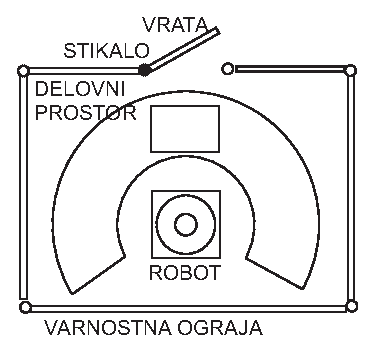
\includegraphics[width=0.60\columnwidth]{fence1.eps}
\end{minipage}
\begin{minipage}[c]{0.5\columnwidth}
\centering
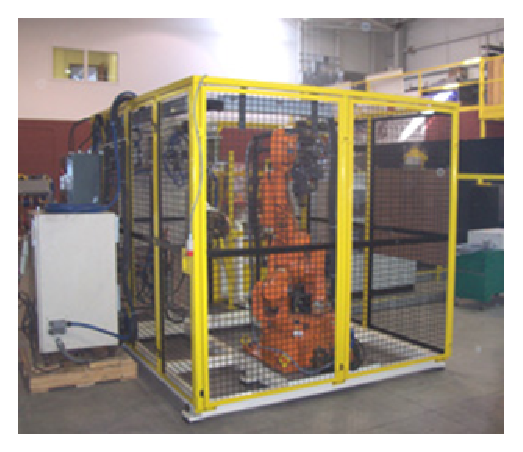
\includegraphics[width=0.9\columnwidth]{fence1_photo.eps}
\end{minipage}
\caption{\label{level1a}Prvi nivo varovanja s fizično ograjo in
vrati}
\end{figure}

\begin{figure}[h]
\begin{minipage}[c]{0.5\columnwidth}
\centering
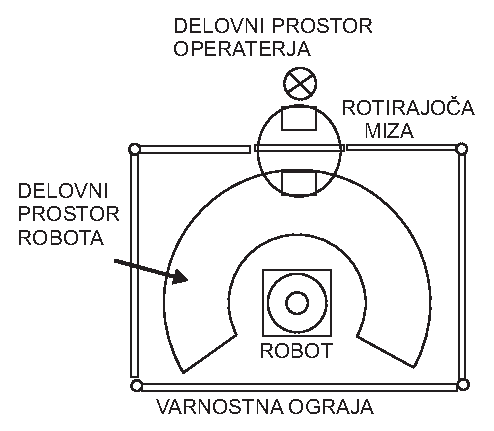
\includegraphics[width=0.80\columnwidth]{fence2.eps}
\end{minipage}
\begin{minipage}[c]{0.5\columnwidth}
\centering
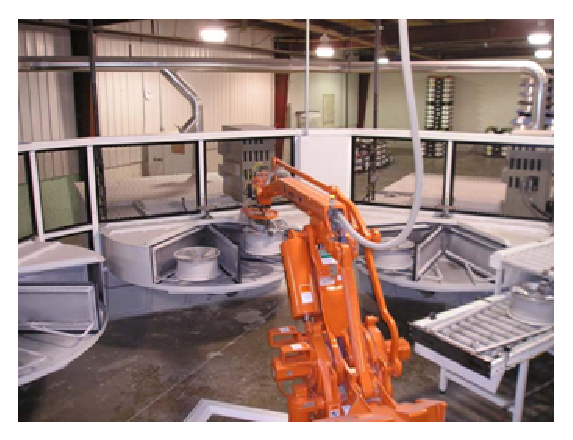
\includegraphics[width=0.9\columnwidth]{fence2_photo.eps}
\end{minipage}
\caption{\label{level1b}Prvi nivo varovanja s fizično ograjo in
rotirajočo mizo}
\end{figure}

\begin{figure}[h]
\begin{minipage}[c]{0.5\columnwidth}
\centering
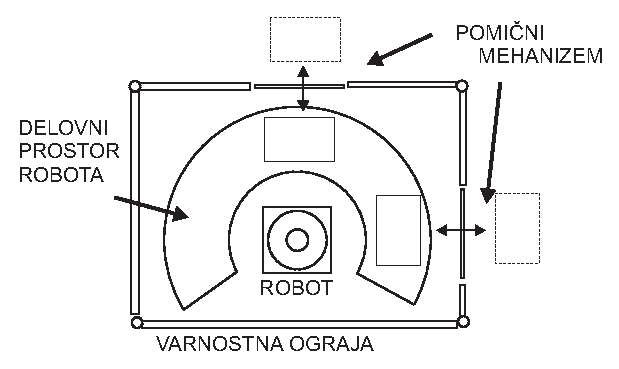
\includegraphics[width=0.90\columnwidth]{fence3.eps}
\end{minipage}
\begin{minipage}[c]{0.5\columnwidth}
\centering
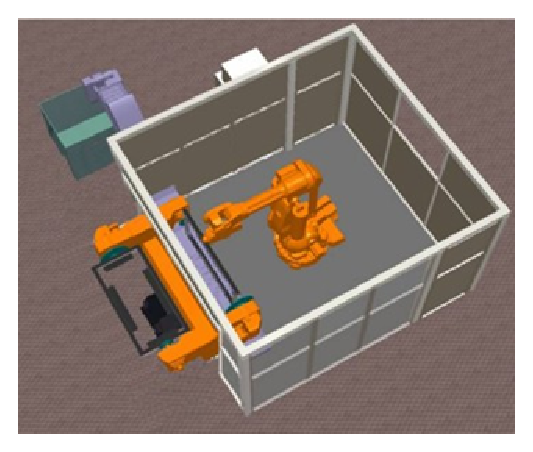
\includegraphics[width=0.9\columnwidth]{fence3_photo.eps}
\end{minipage}
\caption{\label{level1c}Prvi nivo varovanja s fizično ograjo in
pomičnimi mehanizmi}
\end{figure}

%\vspace{5mm}

Na drugem nivoju varovanja pri katerem operater lahko vstopa v
robotsko celico, je varovanje izvedeno na osnovi \textbf{senzorjev
za ugotavljanje prisotnosti operaterja}. To so običajno optični
senzorji, ki delujejo na principu zaznavanja prekinitve žarka,
postavljeni v formacijo optičnih zaves, kot je to prikazano na sliki
\ref{zavesa}. Alternativa je uporaba senzornih preprog, ki na osnovi
izmerjenega tlaka na podlago, zaznavajo položaj operaterja.
\begin{figure}[h]
\centering
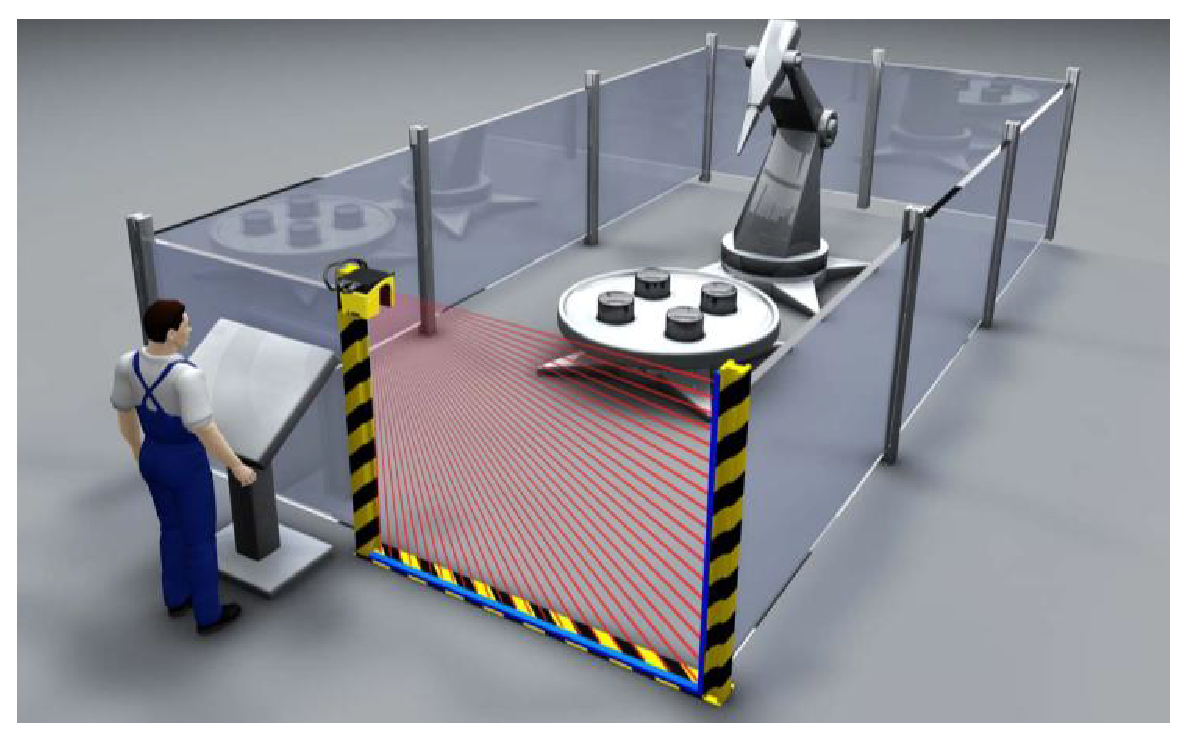
\includegraphics[width=0.7\columnwidth]{zavesa.eps}
\caption{\label{zavesa}Drugi nivo varovanja s pomočjo optičnega
senzorja za zaznavanje prisotnosti operaterja}
\end{figure}

V osnovi naj bi bili senzorji za ugotavljanje prisotnosti
uporabljeni le kot sekundarna oblika zagotavljanja varnosti in to le
v primerih, ko je nujno potreben omejen dostop do robota.

%\vspace{1mm}

Sodobni trendi uporabe robotskih sistemov se razvijajo v smeri
stalnega sodelovanja človeka in robota. Sistem varovanja mora
omogočati hitro prilagajanje robotske celice novim aplikacijam.
Fizično varovanje z mehanskimi ovirami se spreminja v elektronsko
varovanje. Tako so ključni element za zagotavljanje varnosti na
tretjem nivoju senzorji za zaznavanje objektov v delovnem prostoru
robota. Razvijajo se novi optični senzorji, kot so umetni vid in
laserski skenerji. Na sliki \ref{laser_scaner} je predstavljen
laserski skener, ki zaznava prisotnost objektov v različnih merilnih
območjih, s čimer je mogoče programsko določiti in zaznavati kdaj se
človek nahaja v varnem in kdaj v nevarnem območju robotske celice.
\begin{figure}[h]
\begin{minipage}[c]{0.4\columnwidth}
\centering
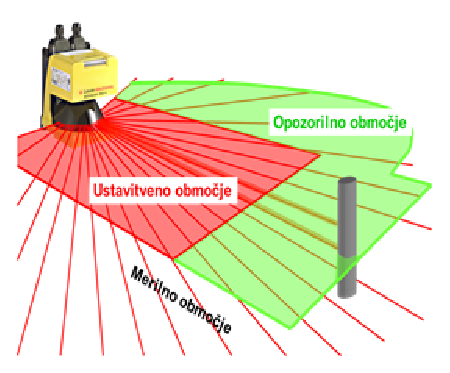
\includegraphics[width=0.98\columnwidth]{laser_scaner_obmocje.eps}
\end{minipage}
\begin{minipage}[c]{0.6\columnwidth}
\centering
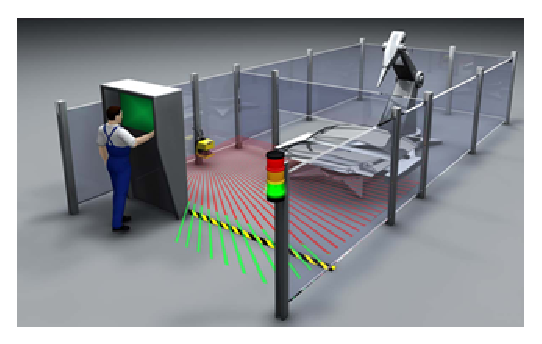
\includegraphics[width=0.98\columnwidth]{laser_scaner.eps}
\end{minipage}
\caption{\label{laser_scaner}Laserski skener za zaznavanje
prisotnosti operaterja s programabilnimi območji zaznavanja}
\end{figure}


\textbf{Senzorji za zaznavanje dotika z robotom} so nameščeni na
robotske segmente ali na vrh robota. Ta pristop se uporablja v
primerih celic z manjšimi roboti, kjer operater med obratovanjem
stoji v bližini robota. Signal, ki ponazarja dotik z robotom,
povzroči hipno izključitev obratovanja robotske celice.

\vspace{5mm}

\textbf{Tipka za izklop v sili} je pomembna pri zagotavljanju
varnosti, saj operaterju omogoča hitro zaustavitev gibanja robota.
Tipka za izklop v sili je nameščena na več mestih v robotski celici
in je nujno velika ter rdeče obarvana, da je lahko opazna in
dosegljiva. Praviloma je nameščena na robotskem krmilniku, na enoti
za ročno učenje ter na ograji robotske celice. Vse varnostne
naprave, kamor spada tudi tipka za izklop v sili, so zaradi čim
hitrejšega izklopa obratovanja s krmilnikom povezane preko ožičene
logike in niso del programske opreme. Sodobni roboti imajo že
vgrajene opcije elektronskega omejevanja gibanja osi (npr. ABB EPS)
ali omejevanja hitrosti gibanja robota ob prisotnosti človeka (npr.
ABB SafeMove).

\vspace{5mm}

Pomembne točke varnostnih priporočil standarda ISO 10218-1, ki
zadevajo nove rešitve varovanja so:
\begin{description}
    \item \vspace*{-0.1cm}5.9 - Priporočila za simultano delovanje več robotov,
    ki določajo pogoje za vodenje več robotskih manipulatorjev z enim krmilnikom.
    \item \vspace*{-0.1cm}5.10 - Zahteve in pogoji za skupno delovanje robota in človeka.
    \item \vspace*{-0.1cm}5.12.3 - Priporočila za programsko omejevanje gibanja
    osi in delovnega prostora, ki omogočajo uporabo elektronskih naprav in programskih
    orodij omejevanja delovnega prostora in hitrosti gibanja robota v smislu zagotavljanja varnosti.
\end{description}
Nov standard ISO 10218-2 (ang. naslov Robots and robotic devices -
Safety requirements Part 2: Industrial robot system and
integration), ki je v pripravi, bo še podrobneje obravnaval
sodelovanje človeka in robota.

\vspace{10mm}

\subsection{Zagotavljanje varnosti pri razvoju programske opreme}

\vspace{5mm}

\textbf{Programiranje in učenje robotskega gibanja} se izvaja s
pomočjo ročnega vodenja robota preko položajev, ki jih robotski
krmilnik pomni in jih nato v avtomatskem načinu izvaja. Za ta
namen je uporabljena enota za ročno učenje. Možno je tudi učenje s
fizičnim vodenjem vrha robota vzdolž trajektorije gibanja, ki si
jo robotski krmilnik zapomni in izvaja. V obeh primerih se mora
operater med učenjem nahajati v robotski celici relativno blizu
robotu. Med učenjem je zato za zagotavljanje varnosti potrebno
biti pozoren na:
\begin{itemize}
    \item \vspace*{-0.1cm} Operater, ki robot uči, mora biti za to
    dobro usposobljen, mora biti seznanjen z vsemi nevarnostmi in
    mora upoštevati ukrepe za zagotavljanje varnosti.

    \item \vspace*{-0.1cm} Med učenjem gibanja se robot ne sme
    gibati z visokimi hitrostmi.

    \item \vspace*{-0.1cm} Operater mora imeti lahek in hiter dostop do tipke za
    izklop v sili.

    \item \vspace*{-0.1cm} Operater mora v vsakem trenutku stati
    na mestu kjer je majhna možnost, da ga robot stisne k fiksnim objektom
    v celici ali da ga poškoduje v primeru okvare.
    Hkrati pa mora poskrbeti, da ima dober pregled nad obratovanjem.

    \item \vspace*{-0.1cm} Priporočljivo je, da je pri učenju
    prisoten opazovalec, ki se nahaja izven delovnega področja
    robota, in ima dostop do takojšnjega izklopa v sili.

    \item \vspace*{-0.1cm} Kjer je to potrebno, mora operater nositi
    zaščitno opremo in zaščitno obleko. Zaščitna čelada je
    obvezna, če obstaja možnost poškodbe glave.

    \item \vspace*{-0.1cm} Ročna učna naprava mora biti takšna, da omogoča gibanje robota samo v primeru, ko operater
    drži posebno tipko.
\end{itemize}


\newpage
\subsection{Zagotavljanje varnosti v Laboratoriju za robotiko na FE Ljubljana}

\vspace{5mm} V Laboratoriju za robotiko in biomedicinsko tehniko
na Fakulteti za elektrotehniko je za varno delo z roboti
poskrbljeno na naslednji način:

\begin{itemize}
    \item \vspace*{-0.1cm} Meje delovnega prostora robotov so
    označene na tleh z rumeno/črnim trakom.

    \item \vspace*{-0.1cm} Operater, ki vstopa v delovni prostor
    mora obvezno nositi zaščitno čelado.

    \item \vspace*{-0.1cm} Na vidnih mestih v vsaki celici se
    nahajajo tipke za izklop v sili.

    \item \vspace*{-0.1cm}Pri poskusnem zagonu se v delovnem
    prostoru ne sme nahajati nihče.

\end{itemize}
